This chapter first discusses the experiments carried out in order to both improve the performance, and gain a better understanding, of the sub-components implemented. Experiments such as hyperparameter optimisation and ablation studies of the two dimensional architecture are discussed. Once the results are cross-validated, the final results achieved by the optimised models are then presented, interpreted, and compared to results achieved by alternative models. Finally, various aspects of the project are critically evaluated.

\section{Two Dimensional Experimentation}

This section reintroduces the initial results achieved by the ``baseline'' two dimensional architecture implemented in Chapter \ref{chap:implementation} and then outlines the experiments carried out in an attempt to improve the performance both qualitatively and quantitatively.

\subsection{Initial Results}

\begin{figure}[!b]
    \begin{subfigure}[b]{0.49\textwidth}
        \centering
        \begin{tikzpicture}[scale=0.9]
            \begin{axis}[
                height=\axisdefaultheight,
                ylabel=\small{Loss},
                xlabel=\small{Epochs},
                ytick={0.15, 0.10},
                yticklabels={0.15, 0.10},
                grid=major,
                legend pos=north east,
                legend cell align=left,
                legend style={fill=white, fill opacity=0.8, draw=none,text opacity=1}]
                \addplot[blue, mark=x] table [x=xs, y=tl, col sep=comma] {csv/base.csv};
                \addlegendentry{\small{Train Loss}}
                \addplot[magenta, mark=x] table [x=xs, y=vl, col sep=comma] {csv/base.csv};
                \addlegendentry{\small{Val Loss}}
            \end{axis}
        \end{tikzpicture}
        \caption{Loss curve}
    \end{subfigure}
    \hfill
    \begin{subfigure}[b]{0.49\textwidth}
        \centering
        \begin{tikzpicture}[scale=0.9]
            \begin{axis}[
                height=\axisdefaultheight,
                ylabel=\small{Accuracy (\%)},
                xlabel=\small{Epochs},
                grid=major,
                legend pos=south east,
                legend cell align=left,
                legend style={fill=white, fill opacity=0.8, draw=none,text opacity=1}]
                \addplot[blue, mark=x] table [x=xs, y=ta, col sep=comma] {csv/base.csv};
                \addlegendentry{\small{Train Accuracy}}
                \addplot[magenta, mark=x] table [x=xs, y=va, col sep=comma] {csv/base.csv};
                \addlegendentry{\small{Val Accuracy}}
            \end{axis}
        \end{tikzpicture}
        \caption{Loss curve}
    \end{subfigure}
    \caption{The loss and accuracy curves achieved when training the model over 20 epochs using the hyperparameters outlined in Table \ref{tab:initialhyperparams}. It is important to note that although the validation loss begins to increase after epoch 13, the validation accuracy does not begin to decrease. Upon visual inspection of the boundary predictions, it could also be seen that the predictions were qualitatively better when the network was trained for 20 epochs rather than 13. The desirable qualitative features of a prediction are outlined in Figure \ref{fig:goodbad}.}
    \label{fig:basetrainacc}
\end{figure}

\begin{figure}[t]
    \centering
    \begin{subfigure}[t]{0.38\textwidth}
        \centering
        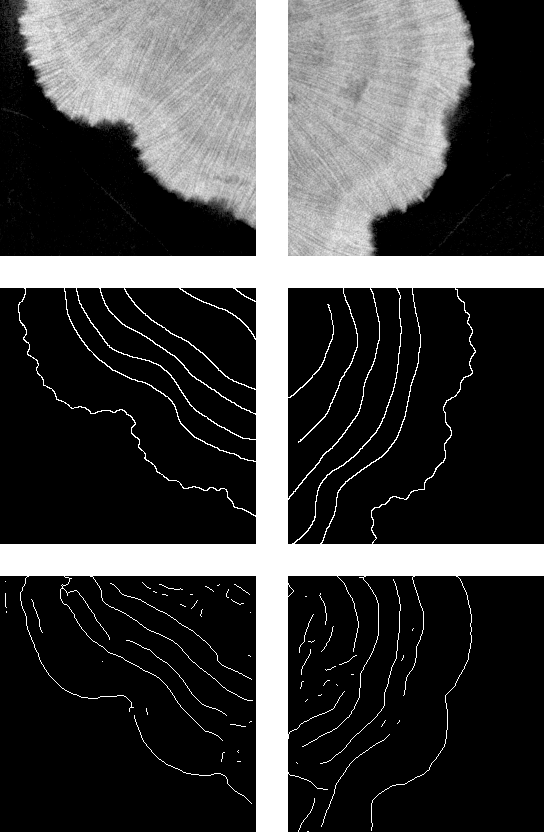
\includegraphics[width=1\textwidth, valign=c]{images/good-initial.png}
        \caption{Higher accuracy: 96.8\% and 96.5\%}
    \end{subfigure}
    ~
    \begin{subfigure}[t]{0.58\textwidth}
        \centering
        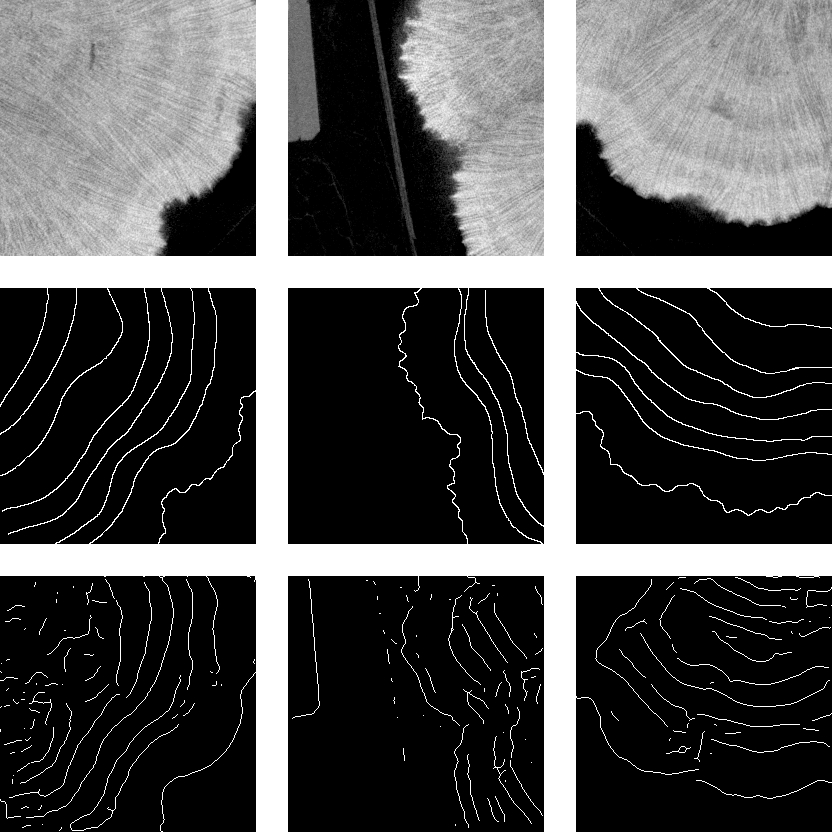
\includegraphics[width=1\textwidth, valign=c]{images/bad-initial.png}
        \caption{Lower accuracy: 92.1\%, 88.4\%, and 91.5\%}
    \end{subfigure}
    \caption{Examples of both high and low quality outputs from the network trained using the initial hyperparameters outlined in Table \ref{tab:initialhyperparams}. The top images are patches from the validation set, the centre images are the corresponding ground truth labels, and the bottom images are the outputs of the network after they have been skeletonized. \textbf{(a)} Examples of high quality predictions. These examples achieved higher accuracies compared to the rest of the samples in the validation set. It can be seen that the boundaries contain comparatively less ``noise'' than the lower quality examples. \textbf{(b)} Examples of low quality predictions. The first example achieves a lower accuracy score due to the noise present in the inner section of the coral (on the left side of the image). The second example received a particularly low accuracy score due to the accidental classification of the object in the top left of the image as a boundary. This object is the platform that the coral sample is placed on in the CT machine and should perhaps have been cropped from the slices that these patches were produced from. The third example receives a low accuracy due to the accidental misclassification of a boundary perpendicular to the skeleton's surface. As discussed in Chapter \ref{chap:context}, density banding boundaries should be parallel to the coral skeleton surface.}
    \label{fig:goodbad}
\end{figure}

The initial results achieved by the baseline model can be discussed further in order to gain a better understanding of the strengths and weaknesses of the model. The loss and accuracy curves are shown in Figure \ref{fig:basetrainacc}, and example boundary predictions of both high and low ``quality'' are shown in Figure \ref{fig:goodbad}. Their quality is assessed both via the accuracy metric achieved and via visual inspection. Looking at Figure \ref{fig:basetrainacc}, it can be see that the accuracy achieved on the validation set is noticeably lower than the accuracy achieved on the training set. This unusual behaviour may be due to the validation set containing ``easier'' examples in which the annual banding is more obvious. Although the performance reported on this validation set may potentially be positively skewed, the final performance achieved by the model will be reported on cross-validated results, and so the selection biases that arise from this dataset split should not affect the final reported performance.

\subsection{Hyperparameter Optimisation}

As discussed in Chapter \ref{chap:technical}, the performance achieved by deep neural networks is known to depend critically on the identification of a good set of hyperparameters~\cite{hyperparam, goodhyperparam}. In this project, a manual form of grid search was used to discover optimised hyperparameter configurations. In this technique, all hyperparameters are fixed and only a single hyperparameter is varied at a time. Although this may not be the most efficient approach, it enables a better understanding of the model to be gained.

% Due to the time constraints of the project, it would not be possible to perform an exhaustive search of all possible hyperparameter configurations. Thus, the primary aim of this chapter is not to achieve the best performance possible, but instead to evaluate which hyperparameters affect the performance most and reason as to why this is the case.

\subsubsection{Learning Rate}

Of all the hyperparameters relevant to deep learning models, the optimisation of the learning rate often has the biggest impact on the performance of a model~\cite{bengio2012practical}. The selection of a learning rate too large can cause an optimisation algorithm to take a step ``over'' minima, causing the loss to inadvertently increase rather than decrease. The selection of a learning rate too small can also hinder performance as the optimisation algorithm may become permanently stuck in a suboptimal local minimum~\cite{goodfellow}.

Since it is usually not possible to calculate an optimal learning rate a priori~\cite{neuralbook}, some form of trial and error is required. A reasonable range of values to experiment with are given by Bengio in~\cite{bengio2012practical} and will be used as the basis of the values experimented with in this section. Bengio suggests an initial learning rate within the range of $10^{-6}$ to $1$.

The accuracies achieved when training the network using various initial learning rates in this range are shown in Figure \ref{fig:lrplot}. It can be seen that the final average accuracy achieved after 20 epochs is similar for all but the 0.00001 value. Although it may look like the accuracy for this learning rate could still improve with further training, the accuracy does not improve further even after 40 epochs. This plateau in the accuracy achieved suggests that the 0.00001 learning rate may be low enough to become stuck in suboptimal local minima.

The training loss achieved by the 0.001 learning rate oscillated at ${\sim}0.5$ for the entire training process, even over multiple training attempts. In comparison, the 0.00005 learning rate achieved a training loss of 0.06 and a validation loss of 0.16. These oscillations are a common sign of a learning rate being too high and stepping ``over'' minima~\cite{bishop1995neural}. Pure black images were output for all samples in both the training and validation sets, resulting in an accuracy of 0\% being achieved.

Although the 0.00005 and 0.0001 learning rates both achieved a similar accuracy of ${\sim}95\%$ after 20 epochs, the 0.00005 value was ultimately chosen for multiple reasons. First, the training and validation accuracy curves are smoother than the curves resulting from higher values, allowing the accuracy to be more reliably used as a stopping criteria for early stopping. Second, when inspecting the results visually, the 0.00005 learning rate results in predictions that are far clearer in the inner areas of the coral skeleton than any other learning rate. Although most of the learning rates were able to produce acceptable predictions nearer to the surface of the coral, only the 0.00005 learning rate was able to produce acceptable predictions in these inner areas. An example of a patch that benefited from the 0.00005 learning rate is shown in Figure \ref{fig:lrdiff}.

\begin{figure}[!t]
    \centering
    \begin{subfigure}[t]{0.32\textwidth}
        \centering
        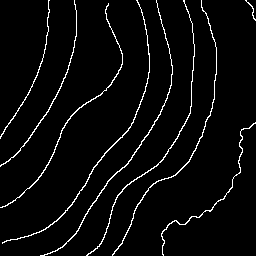
\includegraphics[width=1\textwidth, valign=c]{images/lr-comparison.png}
        \caption{Ground truth boundaries}
    \end{subfigure}
    ~
    \begin{subfigure}[t]{0.32\textwidth}
        \centering
        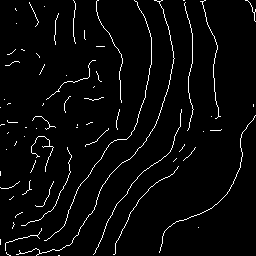
\includegraphics[width=1\textwidth, valign=c]{images/1e4-example.png}
        \caption{$\eta=0.0001$ prediction}
    \end{subfigure}
    ~
    \begin{subfigure}[t]{0.32\textwidth}
        \centering
        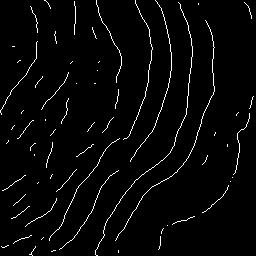
\includegraphics[width=1\textwidth, valign=c]{images/5e5-example.png}
        \caption{$\eta=0.00005$ prediction}
    \end{subfigure}
    \caption{An example of a patch that benefits from the a learning rate $\eta$ of 0.00005. The predictions shown have been skeletonized using the technique discussed in Chapter \ref{chap:implementation}. The $\eta=0.0001$ prediction achieved an accuracy of 92.1\%, whereas the $\eta=0.00005$ prediction achieved an accuracy of 95.5\%. The 0.0001 prediction achieves a lower accuracy score due to the noise present in the inner section of the coral on the left side of the image. The 0.00005 prediction has more realistic predictions in this area of the image with all boundaries almost parallel to the growth surface of the skeleton.}
    \label{fig:lrdiff}
\end{figure}

\begin{figure}[!t]
    \begin{subfigure}[b]{0.49\textwidth}
        \centering
        \begin{tikzpicture}[scale=0.9]
            \begin{axis}[
                height=\axisdefaultheight,
                ylabel=\small{Accuracy (\%)},
                xlabel=\small{Epochs},
                grid=major,
                legend pos=south east,
                legend cell align=left,
                legend style={fill=white, fill opacity=0.8, draw=none,text opacity=1}]
                \addplot[magenta, mark=x] table [x=xs, y=lr00001_vacc, col sep=comma] {csv/lr.csv};
                \addlegendentry{\small{$\eta=0.00001$}}
                \addplot[darkgray, mark=x] table [x=xs, y=lr00005_vacc, col sep=comma] {csv/lr.csv};
                \addlegendentry{\small{$\eta=0.00005$}}
                \addplot[blue, mark=x] table [x=xs, y=lr0001_vacc, col sep=comma] {csv/lr.csv};
                \addlegendentry{\small{$\eta=0.0001$}}
                \addplot[orange, mark=x] table [x=xs, y=lr0005_vacc, col sep=comma] {csv/lr.csv};
                \addlegendentry{\small{$\eta=0.0005$}}
            \end{axis}
        \end{tikzpicture}
        \caption{Varying learning rate}
        \label{fig:lrplot}
    \end{subfigure}
    \hfill
    \begin{subfigure}[b]{0.49\textwidth}
        \centering
        \begin{tikzpicture}[scale=0.9]
            \begin{axis}[
                height=\axisdefaultheight,
                ylabel=\small{Accuracy (\%)},
                xlabel=\small{Epochs},
                grid=major,
                legend pos=south east,
                legend cell align=left,
                legend style={fill=white, fill opacity=0.8, draw=none,text opacity=1}]
                \addplot[magenta, mark=x] table [x=xs, y=bs1_vacc, col sep=comma] {csv/batch.csv};
                \addlegendentry{\small{$batch=1$}}
                \addplot[darkgray, mark=x] table [x=xs, y=bs2_vacc, col sep=comma] {csv/batch.csv};
                \addlegendentry{\small{$batch=2$}}
                \addplot[blue, mark=x] table [x=xs, y=bs4_vacc, col sep=comma] {csv/batch.csv};
                \addlegendentry{\small{$batch=4$}}
                \addplot[teal, mark=x] table [x=xs, y=bs8_vacc, col sep=comma] {csv/batch.csv};
                \addlegendentry{\small{$batch=8$}}
                \addplot[orange, mark=x] table [x=xs, y=bs16_vacc, col sep=comma] {csv/batch.csv};
                \addlegendentry{\small{$batch=16$}}
            \end{axis}
        \end{tikzpicture}
        \caption{Varying batch size}
        \label{fig:bsplot}
    \end{subfigure}
    \caption{The accuracies achieved on the validation set using various hyperparameter values. A TensorBoard smoothing value of 0.3 was used to improve visibility. \textbf{(a)} The accuracies achieved when training the network using various initial learning rate values $\eta$. Apart from varying the learning rate, the same hyperparameters used to achieve the initial results (outlined in Table \ref{tab:initialhyperparams}) were used again here. \textbf{(b)} The accuracies achieved when training the network using various batch sizes. The hyperparameters outlined in Table \ref{tab:initialhyperparams} were used apart from a learning rate of 0.00005.}
\end{figure}

\subsubsection{Batch Size}

The next parameter experimented with was the batch size. Ranging from a size of one up to a few hundreds in some applications~\cite{bengio2012practical}, the batch size not only affects the performance achieved by a network, but can also affect training times significantly.

Small batches with sizes equal to powers of two were experimented with. The accuracies achieved when training using these various batch sizes are shown in Figure \ref{fig:bsplot}. Looking at Figure \ref{fig:bsplot}, it can already be seen that as the batch size increases, the accuracy achieved by the model decreases (with the exception of a batch size of one). Batch sizes greater than 16 were also experimented with but the accuracy achieved only continued to decrease. It may seem that the accuracy achieved when $batch=8$ could increase further given more training epochs. However, even after 40 epochs, the network trained with $batch=8$ only achieved an accuracy of 91\% compared to the accuracy of 95\% achieved when $batch=2$. Note that in order to ensure that the model was exposed to the same number of samples per epoch, with each increase in batch size, the \texttt{steps-per-epoch} argument of the \texttt{fit} method was also decreased. For example, if the batch size was doubled, the \texttt{steps-per-epoch} were halved. This is due to the \texttt{steps-per-epoch} argument specifying how many batches compose an epoch, rather than how many samples compose an epoch.

In practice, it has often been observed that larger batch sizes result in lower accuracy being achieved in deep learning models~\cite{keskar2016large, smallbatch, largebatch}. Keskar et al.\ propose that this decrease in performance may be attributed to larger batch sizes converging to ``sharp'' minima~\cite{keskar2016large}. Whilst a ``flatter'' minimum can be described with low precision, a sharp minimum requires high precision. Keskar et al.\ cite the minimum description length (MDL) theory, which states that statistical models that require fewer bits to describe generalise better~\cite{rissanen}. They argue that since flat minima can be specified with lower precision, they tend to have better generalisation performance. Note that the accuracy achieved on the validation set is a measure of how well the network generalises, since the network has not yet been trained on any slices present in the validation set.

Ultimately, a batch size of two was decided upon as the network trained with this size achieved the highest training and validation accuracy. Although a batch size of 16 provided a ${\sim}1.4$ times speed up in the training process, the model still trains in under 20 minutes when using a batch size of two\footnote{When trained using an Nvidia P100 ``Pascal'' GPU.}. For now, the improved performance provided by a smaller batch size outweighs the benefits provided by the training time saved when using larger sizes. If vast amounts of labelled data were available, a larger batch size would likely be necessary to keep training times reasonable.

\subsubsection{Optimisation Algorithms}

This section discusses experimention carried out with the stochastic gradient descent (SGD) optimisation algorithm. SGD was used successfully to train the original U-Net architecture to perform semantic segmentation on 2D greyscale biomedical data~\cite{ronneberger2015u} and so is a reasonable alternative to the Adam optimiser used so far.

The Keras implementation of SGD using learning rates of 0.00005, 0.0001, 0.0005, 0.001, 0.005, and 0.01 were experimented with but in all cases no acceptable results were produced. When trained with each of these learning rates, the losses and accuracies for both the training and validation sets remained almost constant from the first epoch onwards and the produced predictions resembled the input images more than the corresponding labels. Examples of the predictions produced are shown in Figure \ref{fig:sgdpredictions}.

In an attempt to improve the performance achieved by SGD, various levels of the Keras implementation of classical momentum~\cite{polyak} were experimented with. When momentum is enabled, the weight updates determined by SGD are calculated as a linear combination of the gradient and the previous updates made~\cite{momentum}. Momentum values of 0.1 to 0.9 in combination with all of the learning rates mentioned previously were experimented with but no acceptable results were produced once again. Although no acceptable results were produced, it is important to note that when using a momentum value above 0.5 in combination with a learning rate above 0.001, the validation loss was no longer constant after the first epoch, and a typical loss curve was produced. This suggests that the momentum implemented in Adam may play an important role in allowing the training loss to fall as the training process continues.

Although the SGD optimiser was utilised successfully in the original U-Net paper, the attempts to train this implementation of the architecture using SGD were not successful. Thus, the Adam optimiser continued to be used for the remainder of the experiments.

\begin{figure}[t]
    \centering
    \begin{subfigure}[t]{0.32\textwidth}
        \centering
        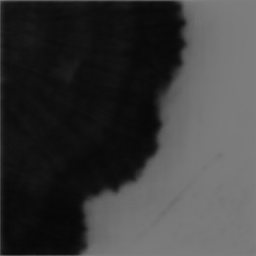
\includegraphics[width=1\textwidth, valign=c]{images/sgd1.png}
    \end{subfigure}
    ~
    \begin{subfigure}[t]{0.32\textwidth}
        \centering
        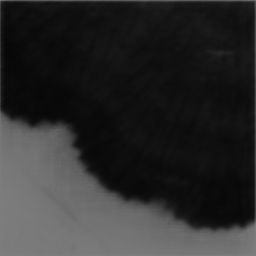
\includegraphics[width=1\textwidth, valign=c]{images/sgd5.png}
    \end{subfigure}
    ~
    \begin{subfigure}[t]{0.32\textwidth}
        \centering
        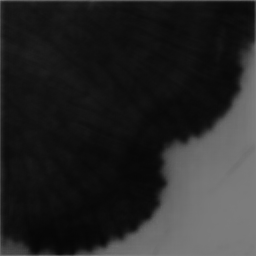
\includegraphics[width=1\textwidth, valign=c]{images/sgd3.png}
    \end{subfigure}
    \caption{Example predictions output by the network when trained using the SGD optimisation algorithm using a learning rate of 0.0001. Predictions almost identical to these were output by all learning rates when a momentum value lower than 0.5 was used. It appears as though the input's channel has been inverted and the image has been blurred slightly.}
    \label{fig:sgdpredictions}
\end{figure}

\subsubsection{Loss Functions}

As outlined in Chapter \ref{chap:implementation}, with ${\sim}$98\% of an average labelled patch being black (part of the ``not part of a boundary'' class), the utilised labelling technique gives rise to a severe class imbalance. As a result, a model that learns to output a pure black image would achieve a low loss value for ${\sim}$98\% of the image. Although this has proved to be a problem when assessing the accuracy of the model, the effects of this class imbalance on the network's ability to learn are not yet obvious. This section outlines the experiments carried out involving the focal loss function~\cite{focalloss} designed specifically to address the class imbalance problem.

The focal loss introduces two tunable parameters: a weighting factor $\alpha \in [0, 1]$ used to increase the loss produced by the misclassification of minority class samples, and a ``focusing'' parameter $\gamma \geq 0$ used to reduce the contribution to the loss that ``easy'' examples have~\cite{focalloss}. When the recommended default values of $\gamma=2$ and $\alpha=0.25$ were used, the network produced predictions comparable to those produced using cross-entropy both qualitatively and quantitatively with a validation accuracy of 93\% being achieved. When varying the $\alpha$ and $\gamma$ parameters, the best accuracy of 94\% was achieved with $\alpha=0.25$ and $\gamma=1$.

When varying the $\gamma$ parameter, an interesting phenomena was observed. Looking at Figure \ref{fig:lossfunctiondiff}, it can be seen that an increase in $\gamma$ results in more pixels being classified as the minority class---the ``part of a boundary'' class. Since the loss value produced per correctly classified black pixel is lower as $\gamma$ increases, the contribution of an incorrectly classified white pixel to the overall loss is far higher. As a result, the network values the correct classification of a white pixel more than the correct classification of a black pixel, and so produces more white pixels overall.

Since even the optimised parameterisation of the focal loss did not yield any improvements over the cross-entropy loss, the cross-entropy loss was ultimately decided upon. The hyperparameters used for the remainder of the experiments are summarised in Table \ref{tab:hyperparams1}.

\begin{table}[t]
    \centering
    \caption{A summary of the training hyperparameters decided upon as a result of the various experiments run.}
    \begin{tabular}{@{}ll@{}}
    \toprule
    Hyperparameter   & Setting      \\ \midrule
    Architecture     & 2D U-Net   \\
    Optimisation Algorithm & Adam \\
    Learning rate & 0.00005 \\
    Loss function & Cross-entropy \\
    Epochs & 20 \\
    Steps per epoch & 500 \\
    Batch size & 2 \\ \bottomrule
    \end{tabular}
    \label{tab:hyperparams1}
\end{table}

\begin{figure}[t]
    \centering
    \begin{subfigure}[t]{0.32\textwidth}
        \centering
        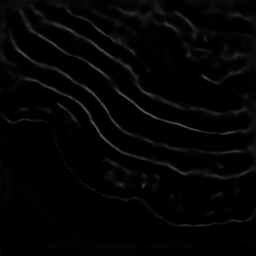
\includegraphics[width=1\textwidth, valign=c]{images/focal_g01.png}
        \caption{$\gamma=0.1$}
    \end{subfigure}
    ~
    \begin{subfigure}[t]{0.32\textwidth}
        \centering
        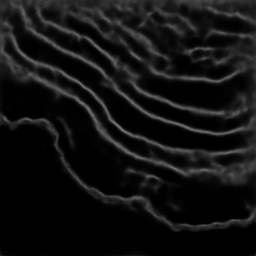
\includegraphics[width=1\textwidth, valign=c]{images/focal_g2.png}
        \caption{$\gamma=2$}
    \end{subfigure}
    ~
    \begin{subfigure}[t]{0.32\textwidth}
        \centering
        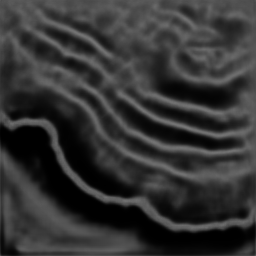
\includegraphics[width=1\textwidth, valign=c]{images/focal_g5.png}
        \caption{$\gamma=5$}
    \end{subfigure}
    \caption{An illustration of how the focusing parameter $\gamma$ of the focal loss function affects the predictions output by the network. Although Lin et al.\ suggest increasing $\alpha$ to 0.75 when $\gamma$ is decreased to 0.1, $\alpha$ was set to a constant value of 0.25 for all values of $\gamma$ to better illustrate how $\gamma$ affects the performance of the network. It can be seen that as $\gamma$ increases, the percentage of pixels that are predicted as the ``part of a boundary'' class also increases.}
    \label{fig:lossfunctiondiff}
\end{figure}

\subsubsection{Dropout Probability}

Dropout is a regularization technique proposed by Srivastava et al.~\cite{dropout} in 2014. As mentioned in Chapter \ref{chap:implementation}, although the original U-Net architecture does not mention any dropout layers, two dropout layers were placed in this implementation: one after the last contracting block and one after the bottleneck block. The experiments carried out in this section involve varying the dropout \texttt{rate} arguments that specify the probability that a neuron is dropped. In the initial implementation, these probabilities were set to 0.5.

The training and validation loss curves resulting from various dropout probabilities are shown in Figure \ref{fig:dropoutplots}. It can be seen that the dropout probability affects the training and validation losses in a similar manner to that discovered by Srivastava et al.; the higher the dropout probability, the higher the training loss and the lower the validation loss~\cite{dropout}.

Similarly to the training loss, the training accuracy also improved as $P$ decreased. However, the validation accuracy was not directly correlated with $P$; the validation accuracies achieved when $P$ was equal to 0.1, 0.3, 0.5, 0.7, and 0.9, were 92\%, 94\%, 95\%, 93\%, and 91\% respectively. Since the validation accuracy was highest when a dropout rate of 0.5 was used, this rate was decided upon.

\begin{figure}[t]
    \begin{subfigure}[b]{0.49\textwidth}
        \centering
        \begin{tikzpicture}[scale=0.9]
            \begin{axis}[
                height=\axisdefaultheight,
                ylabel=\small{Loss},
                xlabel=\small{Epochs},
                grid=major,
                ytick={0.16,0.14,0.12,0.10,0.08,0.06},
                yticklabels={0.16,0.14,0.12,0.10,0.08,0.06},
                legend pos=north east,
                legend cell align=left,
                legend style={fill=white, fill opacity=0.8, draw=none,text opacity=1}]
                \addplot[magenta, mark=x] table [x=xs, y=0_tloss, col sep=comma] {csv/drop.csv};
                \addlegendentry{\small{$P=0.1$}}
                \addplot[darkgray, mark=x] table [x=xs, y=3_tloss, col sep=comma] {csv/drop.csv};
                \addlegendentry{\small{$P=0.3$}}
                \addplot[blue, mark=x] table [x=xs, y=5_tloss, col sep=comma] {csv/drop.csv};
                \addlegendentry{\small{$P=0.5$}}
                \addplot[teal, mark=x] table [x=xs, y=7_tloss, col sep=comma] {csv/drop.csv};
                \addlegendentry{\small{$P=0.7$}}
                \addplot[orange, mark=x] table [x=xs, y=9_tloss, col sep=comma] {csv/drop.csv};
                \addlegendentry{\small{$P=0.9$}}
            \end{axis}
        \end{tikzpicture}
        \caption{Training loss}
    \end{subfigure}
    \hfill
    \begin{subfigure}[b]{0.49\textwidth}
        \centering
        \begin{tikzpicture}[scale=0.9]
            \begin{axis}[
                height=\axisdefaultheight,
                ylabel=\small{Loss},
                xlabel=\small{Epochs},
                grid=major,
                ytick={0.20,0.18,0.16,0.14,0.12},
                yticklabels={0.20,0.18,0.16,0.14,0.12},
                legend pos=north east,
                legend cell align=left,
                legend style={fill=white, fill opacity=0.8, draw=none,text opacity=1}]
                \addplot[magenta, mark=x] table [x=xs, y=0_vloss, col sep=comma] {csv/drop.csv};
                \addlegendentry{\small{$P=0.1$}}
                \addplot[darkgray, mark=x] table [x=xs, y=3_vloss, col sep=comma] {csv/drop.csv};
                \addlegendentry{\small{$P=0.3$}}
                \addplot[blue, mark=x] table [x=xs, y=5_vloss, col sep=comma] {csv/drop.csv};
                \addlegendentry{\small{$P=0.5$}}
                \addplot[teal, mark=x] table [x=xs, y=7_vloss, col sep=comma] {csv/drop.csv};
                \addlegendentry{\small{$P=0.7$}}
                \addplot[orange, mark=x] table [x=xs, y=9_vloss, col sep=comma] {csv/drop.csv};
                \addlegendentry{\small{$P=0.9$}}
            \end{axis}
        \end{tikzpicture}
        \caption{Validation loss}
    \end{subfigure}
    \caption{The loss achieved on the training and validation sets when training the network with varying dropout probabilities $P$. A TensorBoard smoothing value of 0.3 was used to improve visibility. It is important to note that although the validation losses begin to increase after ${\sim}10$ epochs for all dropout probabilities, the validation accuracies and qualitative performance actually continue to improve, and so early stopping before epoch 20 would result in a lower validation accuracy being achieved.}
    \label{fig:dropoutplots}
\end{figure}

% \subsection{Resolution}

% In order to gain a better understanding of the U-Net architecture, the resolution of the patches input to the network was experimented with. These experiments could 
% Even with far more data for smaller patches, the performance was not good. suggests that the network needs context in order to perform well.
% larger slices just did not have enough data but should probably work better using same logic as above?

\subsection{Augmentation}
\label{sec:evalaugmentation}

Due to the little amount of labelled training data available, augmentation proved to be an important regularization technique. The experimentation involving the transformations applied are discussed below. The network was again trained using the hyperparameters summarised in Table \ref{tab:hyperparams1}.

\subsubsection{No Augmentation}

The first experiment involved removing the augmentation process altogether. The \texttt{flow\_from\_directory} method from the \texttt{ImageDataGenerator} class was still used to ensure that shuffling was still performed. The \texttt{steps\_per\_epoch} argument was also still set to 500 batches ensuring that the network was exposed to the same amount of samples throughout the training process. Since there were less than 500 training samples, some of these unaugmented samples were inevitably seen multiple times.

An example prediction output by the network when trained on unaugmented samples is shown in Figure \ref{fig:evalaugnone}. Not only can it be seen that the performance is far worse qualitatively, but an average validation accuracy of 87\% also makes evident the deterioration of the quantitative performance. The validation loss also reached a value of up to 0.4, far higher than the value of 0.15 reached when the network was trained using the initial transformation ranges. It is worth noting that a network trained on a larger dataset would not suffer as big of a deterioration in performance when no augmentation was used, as the dataset itself would already represent a much more comprehensive set of possible samples.

\subsubsection{Augmentation Ranges}

The ranges of acceptable augmentation transformations were also experimented with. The initial ranges outlined in Chapter \ref{chap:implementation} were scaled up and down, and the accuracies and losses achieved were monitored. A phenomena similar to that seen in Figure \ref{fig:dropoutplots} (when the dropout probability was varied) was also observed in this case. The higher the ranges of acceptable transformations, the higher the training loss and the lower the validation loss achieved. The validation accuracy, however, was not directly correlated with the size of the transformation ranges. The highest validation accuracy was achieved using the initial ranges outlined in Chapter \ref{chap:implementation}. Since the initial ranges were selected by hand to be as high as possible whilst also ensuring that the resulting images were ``realistic'', it is understandable that the best performance is achieved when using these ranges. Any higher ranges result in many of the artefacts outlined in Figure \ref{fig:augexample} being present. These artefacts result in augmented samples that no longer represent real coral data, and may be a contributing factor to the lower validation accuracy achieved.

Although higher transformation ranges did result in some valuable qualities being observed in the predictions, a trade-off with other valuable qualities was observed. For example, when looking at Figure \ref{fig:evalaugmentation}, it can be seen that although the highly augmented samples did produce better predictions in the inner areas of the coral skeleton, some degradation in the classification of the ``easier'' boundaries (such as the coral growth surface and the outermost density boundary) is also observed.

Ultimately, the initial ranges outlined in Chapter \ref{chap:implementation} continued to be used as the network trained with these ranges achieved the highest validation accuracy.

\begin{figure}[!t]
    \centering
    \begin{subfigure}[t]{0.24\textwidth}
        \centering
        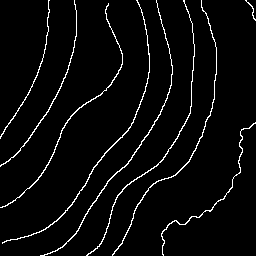
\includegraphics[width=1\textwidth, valign=c]{images/lr-comparison.png}
        \caption{}
    \end{subfigure}
    \begin{subfigure}[t]{0.24\textwidth}
        \centering
        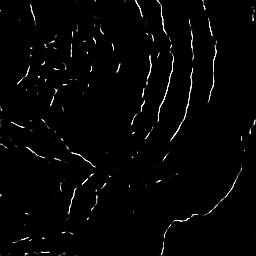
\includegraphics[width=1\textwidth, valign=c]{images/aug-none.png}
        \caption{}
        \label{fig:evalaugnone}
    \end{subfigure}
    \begin{subfigure}[t]{0.24\textwidth}
        \centering
        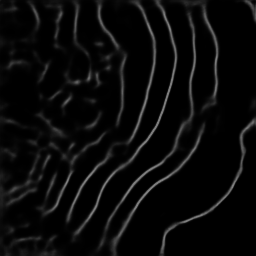
\includegraphics[width=1\textwidth, valign=c]{images/aug-normal.png}
        \caption{}
    \end{subfigure}
    \begin{subfigure}[t]{0.24\textwidth}
        \centering
        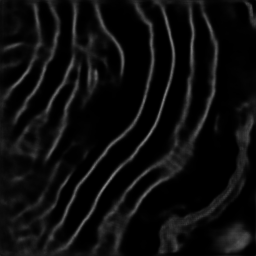
\includegraphics[width=1\textwidth, valign=c]{images/aug-rotation.png}
        \caption{}
    \end{subfigure}
    \caption{Example predictions produced by the network trained using various ranges of acceptable transformations. \textbf{(a)} The ground truth label. \textbf{(b)} A prediction output when no augmentation was used. The network misclassifies the majority of the boundaries, and the continuity within boundaries is often broken. It can also be seen that there are multiple wrongly classified boundaries that are perpendicular to the skeleton's surface. \textbf{(c)} A prediction output when the initial augmentation ranges outlined in Chapter \ref{chap:implementation} were used. \textbf{(d)} A prediction output when the initial ranges outlined in Chapter \ref{chap:implementation} were multiplied by five (e.g., rotations within a range of $\pm 10$ degrees as opposed to $\pm 2$ degrees). Although better predictions in the inner areas of the coral skeleton were produced, some degradation in the classification of the coral growth surface and the outermost density boundary is also observed.}
    \label{fig:evalaugmentation}
\end{figure}

\subsection{Ablation Studies}
\label{sec:evalablation}

In the context of deep neural networks, the term “ablation study” is used to describe a procedure in which certain parts of the network are removed in order to gain a better understanding of the network's behaviour. This section discusses the various ablation studies performed.

\subsubsection{Output Feature Channels Reduction}

The first ablation study involved the removal of varying amounts of the feature channels output by each convolutional layer. When the number of output feature channels were halved for all convolutional layers in all blocks (e.g., the convolutional layer present in the first block now outputs 32 feature channels as opposed to the 64 output by the original architecture), the validation accuracy decreased by ${\sim}2\%$. Despite this decrease only being minor, visual inspection of the resulting predictions showed a noticeable deterioration in their quality. As seen in Figure \ref{fig:ablation}, the main qualitative issue observed was a lack of continuity within the predicted boundaries. Although the boundaries may have been predicted in the right place, many shorter boundaries were predicted rather than the desired long continuous boundaries. This small decrease in accuracy when there is a noticeable decrease in visual quality highlights an issue with the accuracy metric, where breaks in the continuity of boundaries are not punished sufficiently. This issue and other shortcomings of the accuracy metric are discussed further in Section \ref{sec:evalaccuracy}.

Although reducing the output feature channels to half the original amount resulted in a ${\sim}$2.8 times speedup of the training process, the qualitative performance did deteriorate, so the full number of feature channels continued to be used.

\begin{figure}[!t]
    \centering
    \begin{subfigure}[t]{0.24\textwidth}
        \centering
        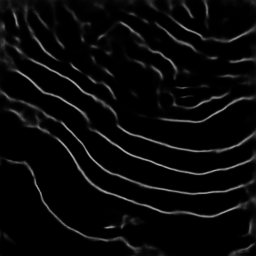
\includegraphics[width=1\textwidth, valign=c]{images/abl-none.png}
        \caption{}
    \end{subfigure}
    \begin{subfigure}[t]{0.24\textwidth}
        \centering
        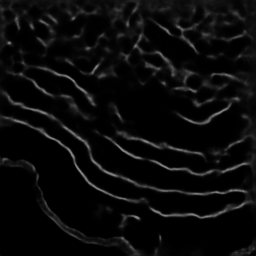
\includegraphics[width=1\textwidth, valign=c]{images/abl-short.png}
        \caption{}
    \end{subfigure}
    \begin{subfigure}[t]{0.24\textwidth}
        \centering
        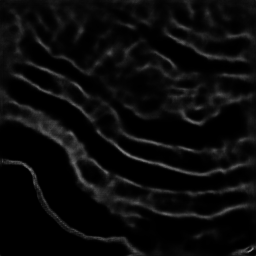
\includegraphics[width=1\textwidth, valign=c]{images/abl-half.png}
        \caption{}
    \end{subfigure}
    \begin{subfigure}[t]{0.24\textwidth}
        \centering
        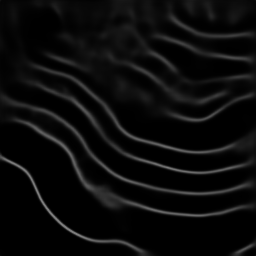
\includegraphics[width=1\textwidth, valign=c]{images/abl-forward.png}
        \caption{}
    \end{subfigure}
    \caption{Example predictions produced by various ablated networks. \textbf{(a)} The prediction output by the unablated network for comparison. \textbf{(b)} A prediction output by the ablated network in which half of the convolutional layers' output feature channels are removed. It can be seen that the continuity within the bands is often broken. \textbf{(c)} A prediction output by the ablated network in which a contracting and expanding block were removed. The boundaries are noisy and blurred in parts. \textbf{(d)} A prediction output by the ablated network with no pass-forward of information. The produced boundaries are significantly smoother and the continuity of the boundaries is rarely broken.}
    \label{fig:ablation}
\end{figure}

\subsubsection{Architecture Shortening}

Another ablation study experimented with the removal of blocks throughout the architecture. In order to maintain the pass-forward of information, the removal of a contracting block also requires the removal of the corresponding expanding block, as this expanding block would otherwise have no contracting block from which information would be passed forward.

When the last contracting block and its corresponding expanding block were removed, the validation accuracy achieved decreased by ${\sim}3\%$ and the produced predictions were noticeably more noisy. This shorter architecture does not contain as many layers and thus the outputs have not been processed by as many operations. The more layers that data has passed through, the ``further'' this data will be from the complex input images. Since the data has not been able to pass through as many layers in this case, the predictions have not been smoothed as much. An example of an output produced by this ablated architecture is shown in Figure \ref{fig:ablation}.

\subsubsection{Max-Pooling Removal}

In order to assess the importance of downsampling in the performance achieved by this architecture, the max-pooling layers in the contracting path and corresponding up-sampling layers in the expanding path were removed. As a result, the feature channels throughout the architecture all have a resolution of 256$\times$256. The ablated network did not perform well as no apparent boundaries were predicted. Blurry images vaguely resembling the input patches were produced and a validation accuracy of 0\% was achieved. It is clear that the downsampling throughout the network is essential for the performance achieved. Since the convolutional layers all had to be applied to full size 256$\times$256 images, training times increased by up to nine times and this ablated network was thus not a viable option anyway.

\subsubsection{Pass-forward Removal}

The final ablation study was used to determine the importance of the pass-forward of information from the contracting path to the expanding path that the U-Net architecture is known for. Other than the removal of all concatenation operations, the rest of the architecture was unchanged. With this pass-forward of information removed, the network performed surprisingly well. Although a decrease in the validation accuracy of ${\sim}1\%$ was observed, the predictions produced were qualitatively better in some respects. When looking at Figure \ref{fig:ablation} for example, it can be seen that the produced boundaries are significantly smoother and that the ``continuity'' of the boundaries is rarely broken. As discussed in Chapter \ref{chap:implementation}, smooth boundaries are deemed as more realistic.

Smoother boundaries may be produced when there is no pass-forward of information from earlier in the network since the data must now pass through the entire network sequentially, and information from feature channels early in the architecture can not be used later on. The feature channels output by the blocks earlier in the architecture will be ``closer'' to the input image, since not as many operations have yet been performed on the data. These earlier feature maps contain images that have not yet been processed by many operations, and thus will not be as smooth as the feature maps output by the last block of the architecture which have had to pass through 26 layers. For example, the U-Net architecture with the pass-forward of information allows the last block of the network to make use of feature channels output by the first block, which have only been processed by two convolutional layers. Whereas, when the architecture does not pass-forward information, the last block can only make use of feature channels that have already passed through 24 layers.

Although smoother boundaries can be seen as a positive quality in this particular task, when performing semantic segmentation with other data, a smoother segmentation is not necessarily more accurate. Note also that padding was used throughout this implementation of the architecture but was not used in the original implementation. This lack of padding in the original implementation by Ronneberger et al.\ significantly reduces the dimensionality of the bottleneck and could significantly affect the performance achieved when no pass-forward of information is present. Thus, although the lack of any pass-forward of information did not deteriorate the performance achieved in this task, the pass-forward may still be valuable when the architecture is implemented differently or utilised for different segmentation tasks.

The performances achieved by the various ablated networks are summarised in Table \ref{tab:ablation}. Ultimately, due to the smoother continuous boundaries produced, the pass-forward of information was in fact removed and the resulting ablated network was used for the results shown in Section \ref{sec:finalresults}.

\begin{table}[!t]
    \centering
    \caption{A summary of the performances achieved by the various ablated networks discussed throughout this section. Note that the unablated network took ${\sim}16$ minutes to train on an Nvidia P100 ``Pascal'' GPU.}
    \begin{tabular}{@{}lrrrr@{}}
\toprule
Ablation                  & Trainable Parameters & Speedup     & Validation Accuracy \\ \midrule
None                      & 31,031,685           & $\times1.0$ & 95\%                \\
Pass-forward Removal      & 27,898,245           & $\times1.1$ & 91\%                \\
Feature Channel Reduction & 7,760,069            & $\times2.8$ & 93\%                \\
Architecture Shortening   & 7,697,285            & $\times1.5$ & 92\%                \\
Max-Pooling Removal       & 31,031,685           & $\times0.1$ &  0\%                \\ \bottomrule
\end{tabular}
    \label{tab:ablation}
\end{table}

\section{Alternative Three Dimensional Architectures}

This section discusses the experiments carried out involving the structure of the three dimensional architecture implemented in Chapter \ref{chap:implementation}.

% \subsection{3D to 2D Architectures}

% The initial modified architecture implemented in Chapter \ref{chap:implementation} took three dimensional samples as input (in the form of nine two dimensional patches) and attempted to produce some two dimensional output (the prediction of the boundary positions in the central patch). Various other ``3D to 2D'' architectures were also experimented with and are discussed below.

\subsection{Increased Convolutional Output Channels}

As mentioned in Chapter \ref{chap:implementation}, the number of feature channels output by the 3D convolutional layers were chosen in an attempt to replicate the original 2D U-Net architecture as closely as possible. Initially, the number of output channels was chosen to be eight times less than the number of output channels used in the 2D architecture (i.e., since the first block of the 2D architecture output 64 feature channels, only eight were output by the 3D architecture). The output feature channels must be reshaped in order to be used with 2D layers, resulting in the number of output channels being multiplied by nine. Thus, a factor of eight was the closest factor that divided evenly into the numbers of output feature channels used in the original paper (e.g., 64, 128, 256, etc.).

Whilst experimenting with the number of output feature channels, it was found that a higher number of feature channels (e.g., dividing by a factor of four rather than a factor of eight) produced significantly worse qualitative results and the validation accuracy dropped from ${\sim}$77\% to ${\sim}$43\%. The noticeably better performance achieved when using fewer output feature channels may be due to the reduction in the number of trainable parameters acting as a regularization technique.

% \subsubsection{Simple extension of the 2D U-Net}

% Another architecture experimented with consisted of the original 2D U-Net with a small amount of 3D convolutional layers placed at the start. These 3D convolutional layers allow the network to make use of the extra information available in the third dimension before the feature maps are reshaped and passed into the 2D architecture. Varying numbers of convolutional layers, numbers of output feature channels, and kernel sizes were experimented with but n

% original version with a few 3d convs on the front and then outputting to a 2D (9 channels or 1) image to put straight into U-Net. May not have worked due to vanishing gradients? its right at the beginning of the network?

\subsection{Fully Three Dimensional Architecture}
\label{sec:eval3darch}

A fully three dimensional U-Net architecture was also experimented with. Similarly to the architectures discussed previously, this architecture also takes a chunk of nine patches as input. However, rather than only attempting to predict the boundaries present in the central slice, this architecture attempts to predict the boundaries present in all nine patches. Since the network is learning to label every input patch, the labels for these patches must also be provided.

Thus, in order to train the fully three dimensional architecture with the same amount of samples used previously, up to nine times as many slices would have to be labelled. This was not a realistic goal within the time frame of this project and only a small amount of adjacent slices were ultimately labelled. Two sets of nine slices that were all adjacent to each other were labelled, and the sliding window technique described in Chapter \ref{chap:implementation} was used once again to curate a small three dimensional dataset. Using the custom data loader detailed in Chapter \ref{chap:implementation}, the three dimensional architecture was trained on various augmented versions of these three dimensional samples. Unfortunately, the architecture ultimately performed poorly, with the output predictions containing almost no visible boundaries.

Although this architecture performs poorly for various reasons, the lack of labelled three dimensional data may be the most significant. When looking at the training and validation loss curves, it can be seen that whilst the training loss continues to decrease for all 20 epochs, the validation loss begins to increase after only the second epoch. It appears as though the lack of data may be causing the network to severely overfit.

The quality of the labelled three dimensional data may be also be contributing to the poor performance achieved. As mentioned in Chaper \ref{chap:implementation}, labelling the boundaries consistently is challenging. Looking at Figure \ref{fig:3dlabel}, it can be seen that the adjacent slices may not have been labelled consistently. Although the two labels are clearly similar, it is important to note that the slices that these labels correspond to are near identical, since the two slices are adjacent and are each only ${\sim}$0.1 mm thick. The corresponding labels cannot realistically be more than one pixel apart from each other at any point. As the network was trained on these inconsistent nine-patch labels, it may have struggled to determine any relationships within the third dimension of the data. If the use of three dimensional architectures to extract these boundaries is revisited, consistent labelling of adjacent slices will be necessary if acceptable performance is to be achieved.

It is worth noting that although the hyperparameters outlined in Section \ref{sec:threedimension} were initially used, multiple combinations of different learning rates, batch sizes, dropout rates, and kernel sizes were also experimented with, but none produced any visible boundaries. Ultimately, the original architecture whose implementation is discussed in Chapter \ref{chap:implementation} achieved the best performance of any of the three dimensional architectures experimented with.

\begin{figure}[t]
    \centering
    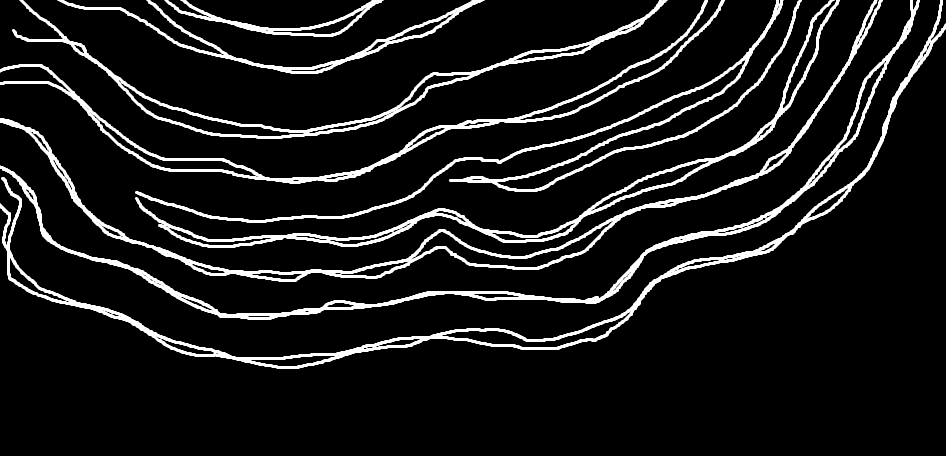
\includegraphics[width=0.8\textwidth]{images/3D-label-example.png}
    \caption{An example of two inconsistent adjacent labels. Lines corresponding to the same boundary in both slices can be up to eight pixels apart at some points. In reality, these boundaries should be no more than one pixel apart at any point.}
    \label{fig:3dlabel}
\end{figure}

\section{Cross-validation}
\label{sec:evalcrossval}

As outlined in Chapter \ref{chap:technical}, cross-validation techniques are used to give a comprehensive measure of a model's performance throughout the entire dataset, rather than just a particular subset. Cross-validation techniques reduce the effects of selection bias on the reported performance. Since the slices composing the test set and the slices composing the training set were extracted from different samples, some form of selection bias is inevitable and the performance achieved on the current test set does not necessarily represent the performance that would be achieved on the entire dataset.

\subsection{Train/test Splits}

In order to perform cross-validation, the dataset must be split into multiple training and testing sets known as ``train/test'' splits. Similarly to how the dataset was split in Chapter \ref{chap:implementation}, the patches composing the test sets must all be produced from slices of coral skeletons that are not part of the corresponding training sets. This ensures that in each train/test split, the network cannot be overfitting to the nature of the annual banding present in the skeletons used for testing. If this had been the case, the performance on each test set could have been positively skewed. For this reason, the train/test splits were manually selected, as opposed to randomly selected as they usually can be. It is important to note that no hyperparameters or augmentation settings were changed during the cross-validation process, as this could have been used to influence the final reported performance in some way.

Since all of the data was extracted from four coral skeletons, four splits were selected. In each split, the test set consists of every patch produced from one skeleton, and the training set consists of every patch produced from the rest of the available skeletons. The accuracies achieved for each train/test split are shown in Table \ref{tab:crossval}.

\begin{table}[!t]
    \centering
    \caption{The accuracies achieved on the various cross-validation splits.}
    \begin{tabular}{@{}lrrr@{}}
\toprule
Test scan & Training samples & Test samples & Accuracy \\ \midrule
RS0030    &                  &              &          \\
RS0116    &                  &              &          \\
RS0128    &                  &              &          \\
RS0130    &                  &              &          \\ \midrule
Average   &                  &              &          \\ \bottomrule
\end{tabular}
    \label{tab:crossval}
\end{table}

\section{Final Results}
\label{sec:finalresults}

This section introduces and discusses the final results achieved by the ablated two dimensional architecture described in Section \ref{sec:evalablation}. The estimated calcification rates for each of the coral skeletons are also presented.

\subsection{Final Boundary Extraction Results}

Examples of higher and lower quality predictions produced by the final ablated two dimensional architecture are shown in Figures \ref{fig:finalresultsgood} and \ref{fig:finalresultsbad} respectively. The final cross-validated accuracy achieved was 77.8\%.

Looking at Table \ref{tab:crossval}, it can be seen that the split in which RS0030 is the test scan achieves the highest accuracy. This better performance achieved may be due to the validation set that was chosen to perform hyperparameter optimisation with. Since the slices composing the validation set were all extracted from the RS0030 scan, the hyperparameters were optimised in order to maximise the performance on this scan. However, it is also worth noting that the RS0030 scan contains arguably the most obvious annual banding, and so the better performance achieved may also be due to the RS0030 scan being inherently ``easier''. The banding present in this skeleton is more easily identified because the changes in density at the boundaries of two bands are often more abrupt---the density changes quickly over the space of only a few pixels. With other skeletons, however, the changes in density are often more gradual, and are thus harder to discern.

The slightly lower accuracy achieved on the RS0116 split may be due to the lack of training data available. Since the majority of the patches composing the curated dataset were extracted from this scan, only 128 training patches remained. Unfortunately, when classifying the RS0130 testing set, only the coral growth surfaces were ever successfully classified as a boundary. As a result, a significantly lower accuracy of 36.6\% was achieved. Although it is unclear exactly as to why the network performed so poorly on this test set, it is worth noting that the annual banding present in the RS0130 scan was particularly hard to label manually. It was expected that the network would perform worse on this scan, nevertheless the lack of any boundaries being detected at all was a particularly poor result.

\begin{figure}[!p]
    \centering
    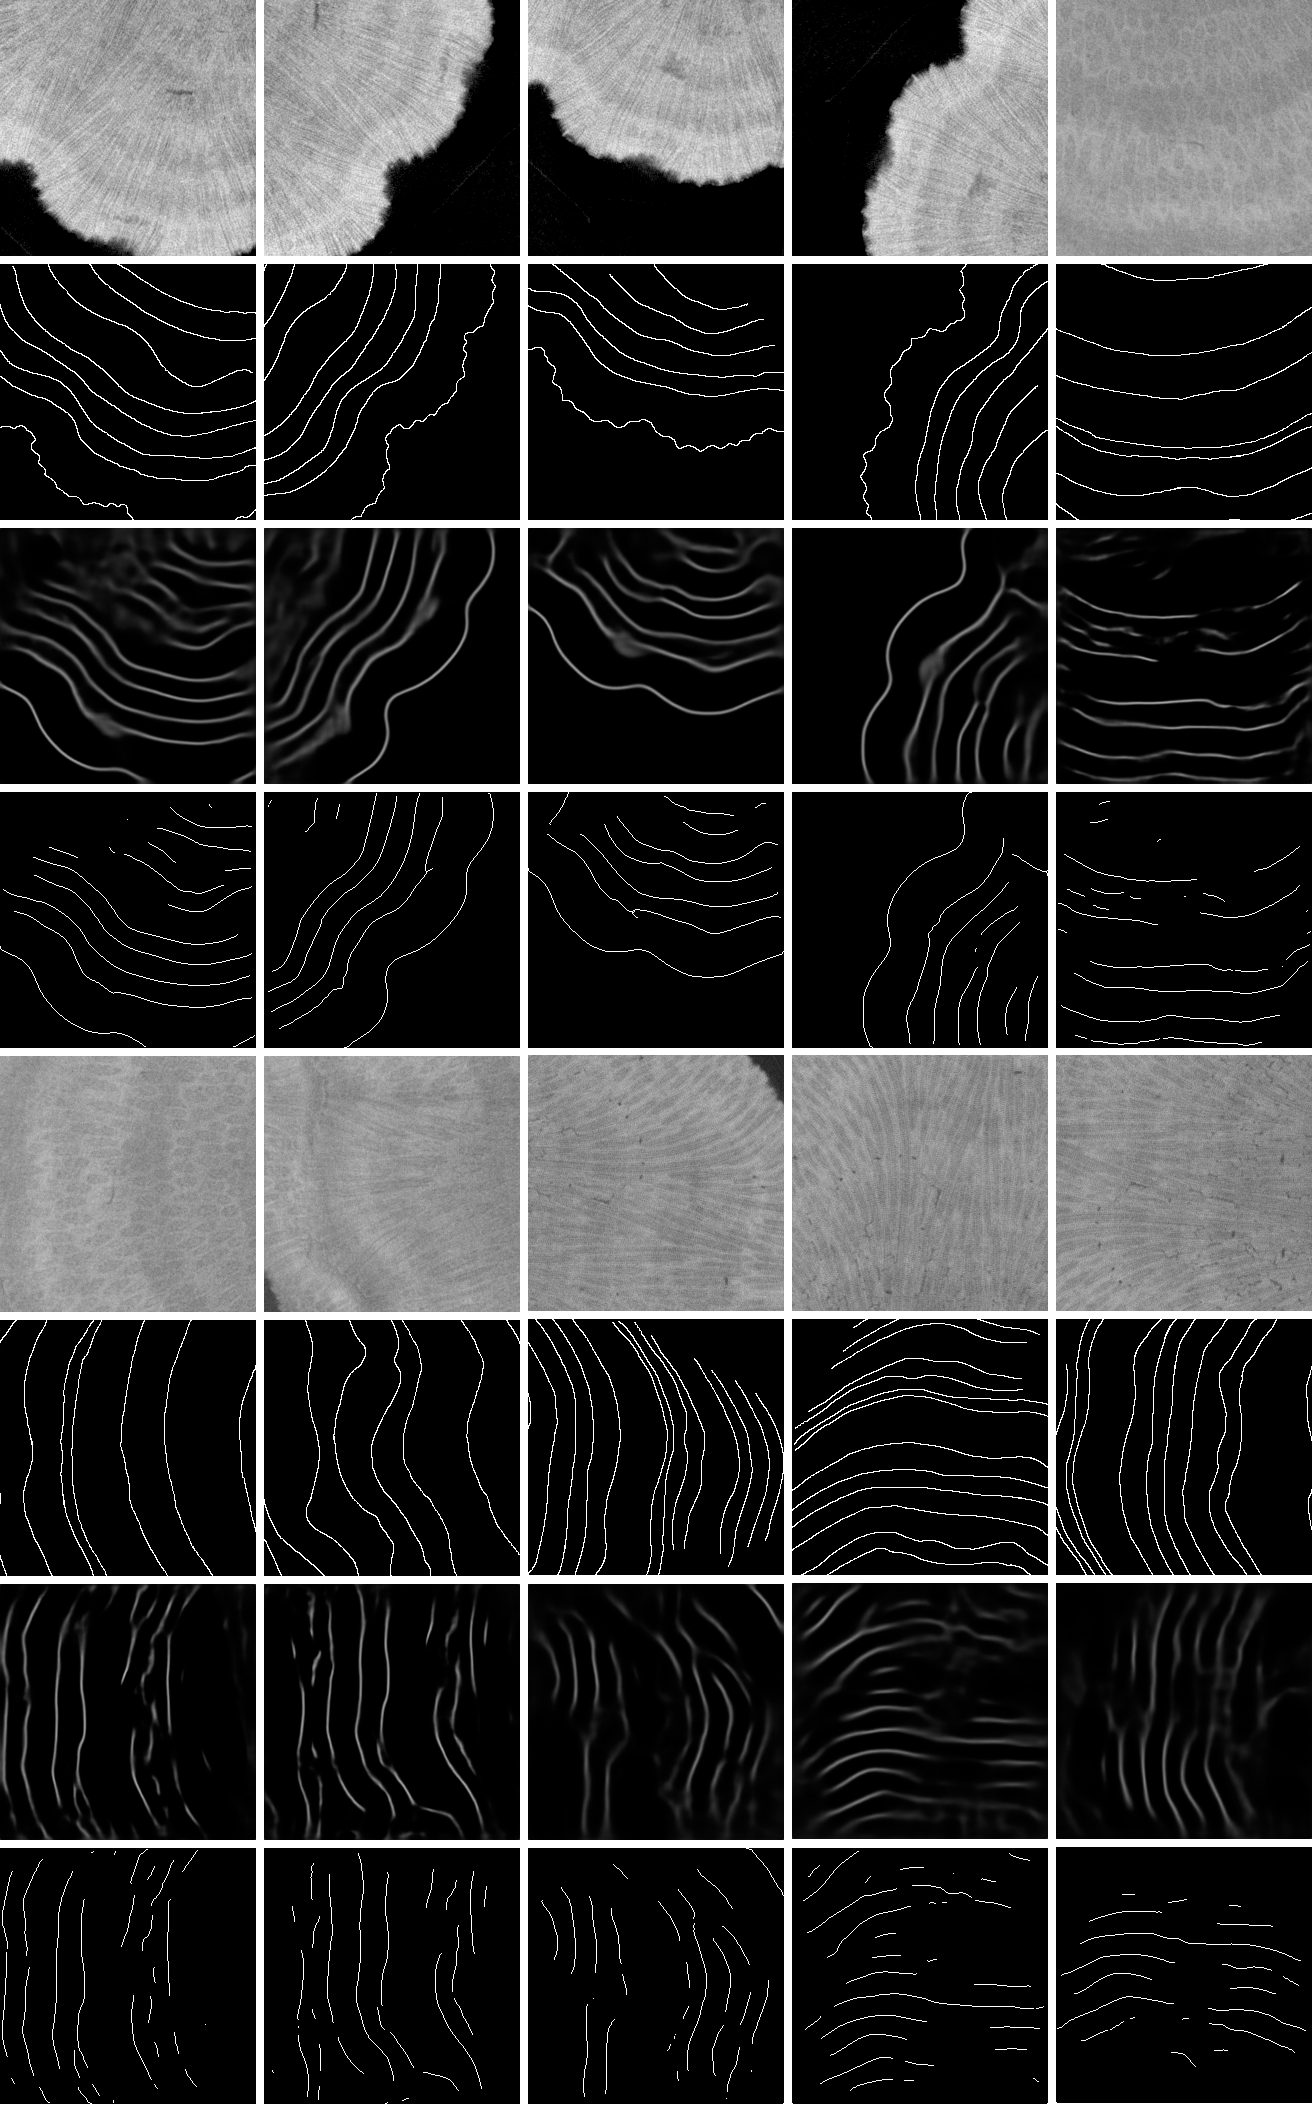
\includegraphics[width=0.91\textwidth]{images/final-results-good.png}
    \caption{Higher quality examples of the final predictions produced by the network. From top to bottom: image, label, prediction, skeletonized prediction.}
    \label{fig:finalresultsgood}
\end{figure}

\begin{figure}[!p]
    \centering
    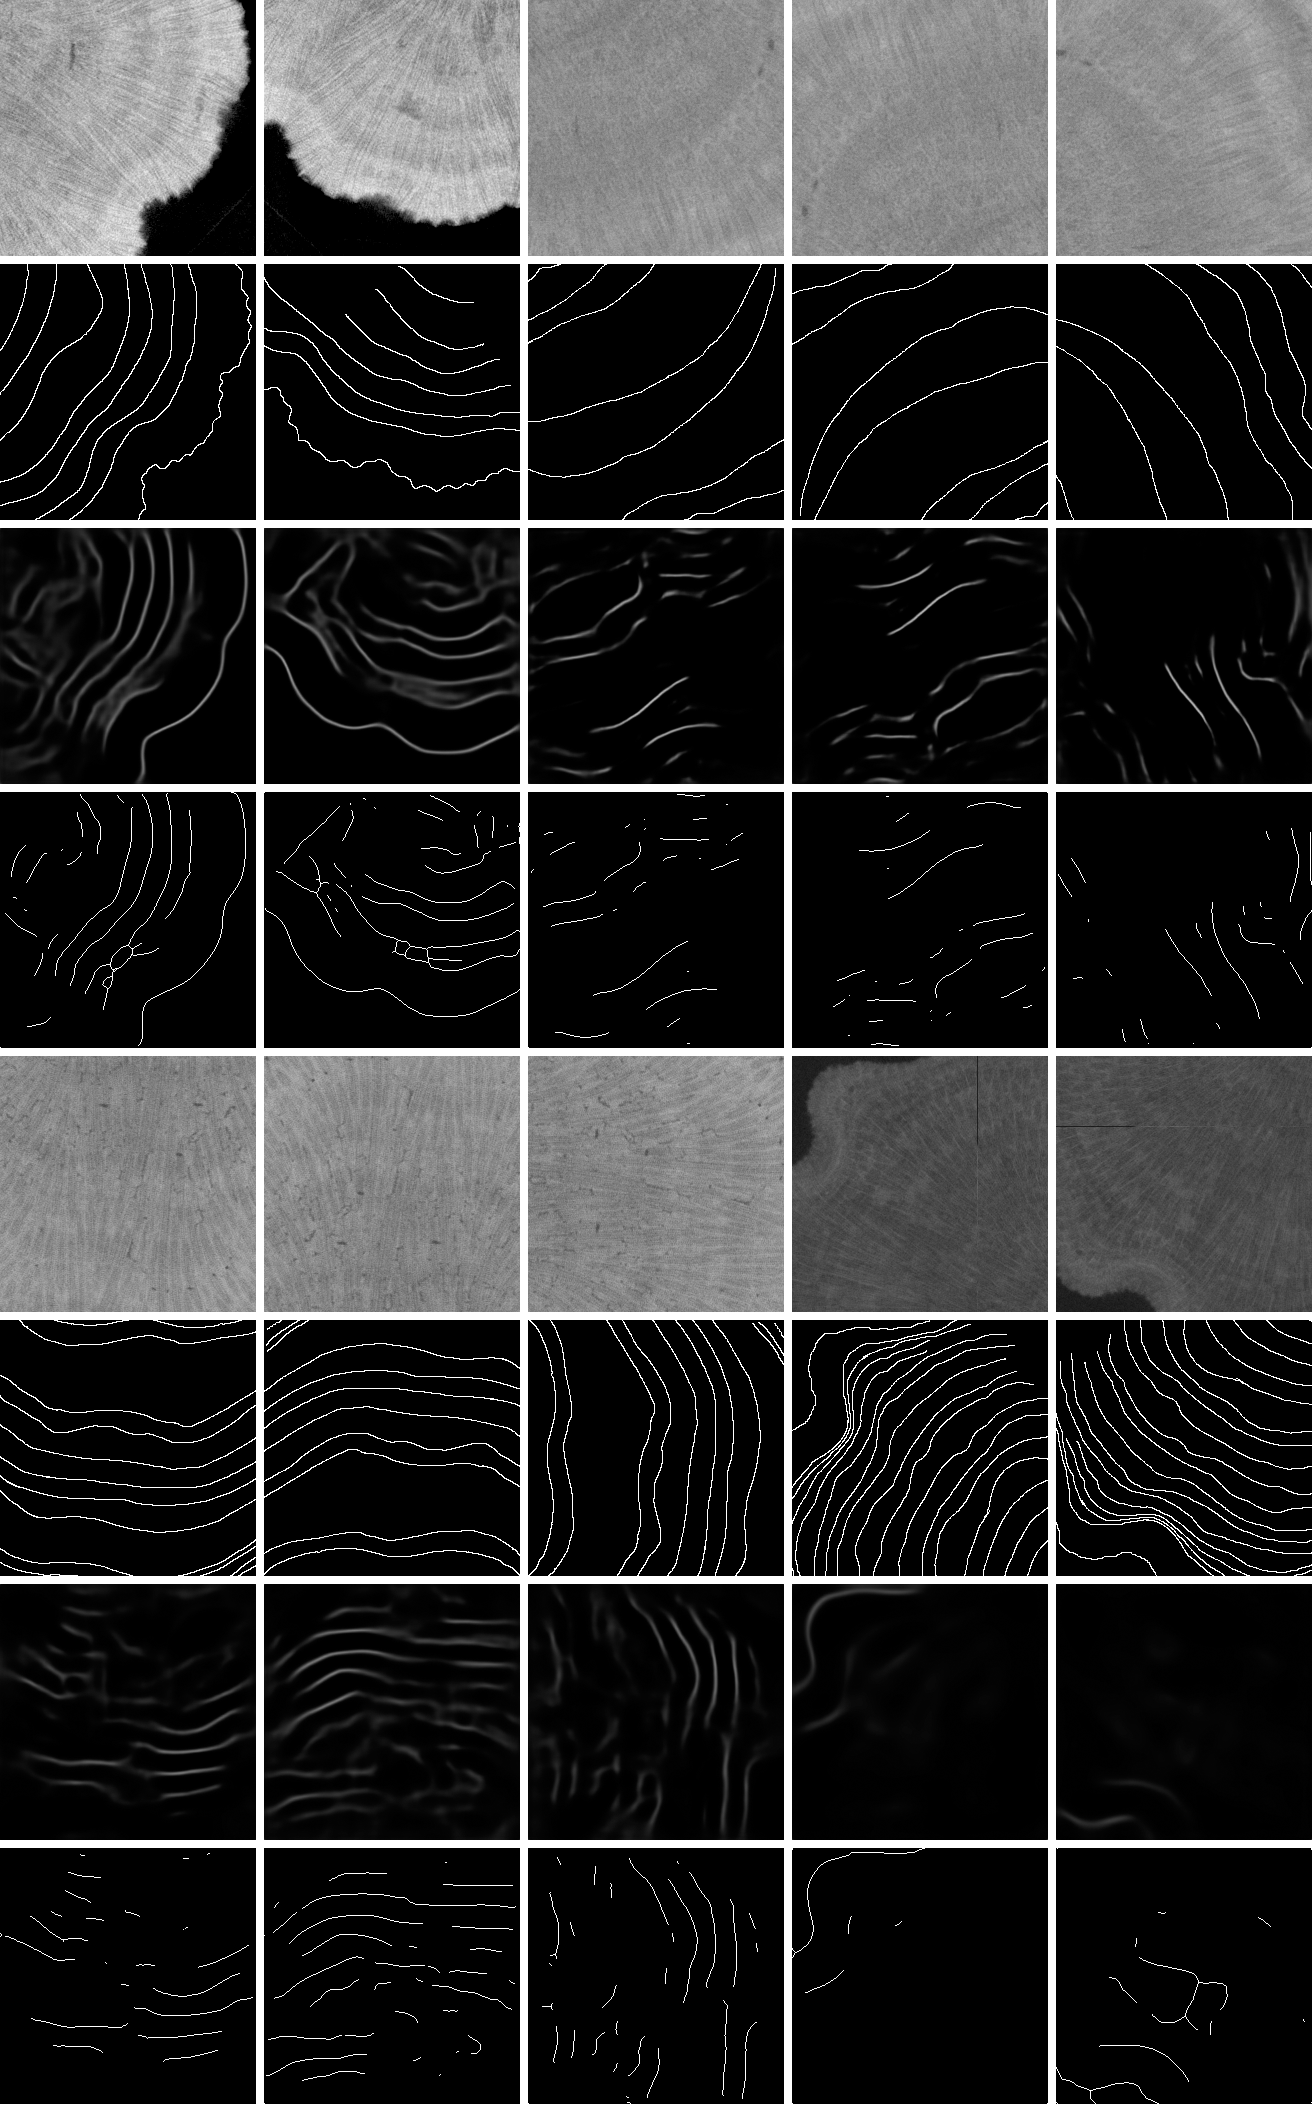
\includegraphics[width=0.91\textwidth]{images/final-results-bad.png}
    \caption{Lower quality examples of the final predictions produced by the network. From top to bottom: image, label, prediction, skeletonized prediction.}
    \label{fig:finalresultsbad}
\end{figure}

\subsection{Final Calcification Rate Estimates}

The density, linear extension rate, and calcification rate estimates made using the Python script described in Section \ref{sec:calcificationimplementation} are listed in Table \ref{tab:calcification}. The estimates made using both the ground truth boundaries and the predicted boundaries are shown.

These automatic estimates for Porites skeletons are in line with the manual estimates reported in the literature \cite{calcification1, calcification2}. The average calcification rate of 0.51 g cm$^{-2}$ y$^{-1}$ found using the components implemented in this project is also similar to the calcification rate manually estimated by researchers at the Natural History Museum\footnote{According to values provided by Dr Kenneth Johnson, an average calcification rate of 0.48 g cm$^{-2}$ y$^{-1}$ was found on the samples that compose the dataset used to train the network.}.

% For example, \cite{calcification1} reports averages of 1.17 g cm$^{-3}$, 5.70 cm y$^{-1}$, and 0.65 g cm$^{-2}$ y$^{-1}$ for the density, LER, and CR respectively, whilst \cite{calcification2} reports averages of 1.08 g cm$^{-3}$, 4.70 cm y$^{-1}$, and 0.51 g cm$^{-2}$ y$^{-1}$.

% 2.9 * 1.16 = 0.33
% 3.66 * 1.52 = 0.55

\begin{table}[!t]
    \centering
    \caption{The density, linear extension rate, and calcification rate estimates produced using the Python script described in Section \ref{sec:calcificationimplementation}. The estimates produced when using the ground truth boundaries are compared with the estimates produced when using the boundaries predicted by the final ablated two dimensional architecture. Note that the network did not produce any valid boundaries for the RS0130 scan so the corresponding estimates are left blank. The average linear extension rate and the average calcification rate estimated using the predicted boundaries are higher as a result.}
    \small
    \begin{tabular}{@{}lrrrrrr@{}}
\toprule
         & \multicolumn{2}{c}{\textbf{Density (g cm$^{-3}$)}} & \multicolumn{2}{c}{\textbf{Linear extension rate (mm y$^{-1}$)}} & \multicolumn{2}{c}{\textbf{Calcification rate (g cm$^{-2}$ y$^{-1}$)}} \\ 
         &                             &                      &  \quad\quad\quad    Label &       Prediction\quad\quad\quad\quad &        \quad\quad\quad    Label &       Prediction\quad\quad\quad\quad \\ \midrule 
RS0030   &          \multicolumn{2}{c}{1.68}                  &                     4.14  &             4.24\quad\quad\quad\quad &                            0.70 &             0.71\quad\quad\quad\quad \\
RS0116   &          \multicolumn{2}{c}{1.52}                  &                     5.26  &             5.15\quad\quad\quad\quad &                            0.80 &             0.79\quad\quad\quad\quad \\
RS0128   &          \multicolumn{2}{c}{1.74}                  &                     2.90  &             3.02\quad\quad\quad\quad &                            0.51 &             0.53\quad\quad\quad\quad \\
RS0130   &          \multicolumn{2}{c}{0.94}                  &                     2.08  &               --\quad\quad\quad\quad &                            0.20 &               --\quad\quad\quad\quad \\ \midrule
Average  &          \multicolumn{2}{c}{1.47}                  &                     3.60  &             4.14\quad\quad\quad\quad &                            0.51 &             0.67\quad\quad\quad\quad \\ \bottomrule
\end{tabular}
    \label{tab:calcification}
\end{table}

\section{Comparisons with Other Architectures}

This section outlines the experimentation carried out involving various other architectures that can be utilised to perform semantic segmentation. Comparing the performances achieved by similar architectures can help one gain a better understanding of which aspects of the architectures affect performance the most.

\subsection{SegNet}

The first architecture experimented with was SegNet~\cite{segnet}. It was implemented using Keras, enabling it to be easily integrated into the code used in this project. The implementation is based heavily off of an implementation available on GitHub\footnote{\url{https://github.com/ykamikawa/tf-keras-SegNet}}, which follows the architecture outlined in the original paper very closely. The learning rate and batch size were briefly experimented with, and in this case, a learning rate of 0.0001 and a batch size of two were found to produce the best results of any combination tested.

An example of a prediction produced by the SegNet implementation is shown in Figure \ref{fig:segexample}. It can be seen that although some banding was correctly identified in the bottom right of the prediction, the qualitative performance is poor overall. This is reflected by a validation accuracy of only 56\% being achieved.

As mentioned in Chapter \ref{chap:technical}, the U-Net and SegNet architectures are remarkably similar overall. Both architectures follow some form of fully convolutional encoder-decoder structure and utilise some form of pass-forward of information from encoding blocks early in the architecture to decoding blocks later on. The similarity of the underlying fully convolutional encoder-decoder structures suggests that perhaps the difference in performance between the two architectures arises from the different methods of pass-forward used. Although the pass-forward of information is removed in the final architecture used in this project, the unablated U-Net architecture still performs significantly better than the SegNet architecture. The SegNet architecture passes information forward in the form of pooling indices. When this pass-forward of information was removed, the architecture performed better both qualitatively and quantitatively, with a validation accuracy of 75\% now being achieved. This suggests that perhaps the passing forward of pooling indices is not as useful in this task as it is in other semantic segmentation tasks.

It is worth noting that the results discussed here may not be a true representation of the SegNet architecture's potential, as more time was spent optimising the hyperparameters used with U-Net architecture. The hyperparameter settings used to achieve these results are summarised in Table \ref{tab:segnetparams}.

\subsection{pix2pix}

The pix2pix model~\cite{pix2pix} has shown some success whilst performing semantic segmentation and was an interesting model to experiment with. The experiments were carried out using a PyTorch\footnote{\url{https://pytorch.org}} implementation provided by the original authors\footnote{\url{https://github.com/junyanz/pytorch-CycleGAN-and-pix2pix}}. The generator was trained to generate boundary labels given some coral skeleton patches. The default hyperparameters specified by the authors were used and are summarised in Table \ref{tab:pix2pixparams}.

An example of a label generated is shown in Figure \ref{fig:pixexample}. It appears as though the generator produces almost random predictions. Although at first glance these predictions look feasible, upon closer inspection it can be seen that the boundaries being predicted are completely wrong in many respects. In most of the labels produced, the predicted boundaries are not parallel to the growth surface and the spaces between them are significantly different than the spaces that exist between the ground truth labels. It is not obvious what data the generator is using to generate these labels, as no relationships between the patches and the generations can be found via visual inspection.

It is not clear as to why the pix2pix model performs so poorly at this task. Since the generator is only trained to maximise the probability that the discriminator makes a mistake, perhaps the discriminator is already not able to discern these fake labels from the real ones, and so the generator is not incentivised to generate labels that are any more realistic. Ultimately, the model achieved a validation accuracy of 37\%. Note that the results discussed here may not be a true representation of the pix2pix model's potential, as more time could be spent optimising the hyperparameters used with the model and the performance achieved could improve.

\begin{figure}[!t]
    \centering
    \begin{subfigure}[t]{0.24\textwidth}
        \centering
        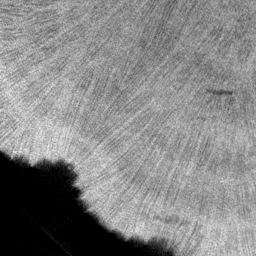
\includegraphics[width=1\textwidth, valign=c]{images/5_image.png}
        \caption{}
    \end{subfigure}
    \begin{subfigure}[t]{0.24\textwidth}
        \centering
        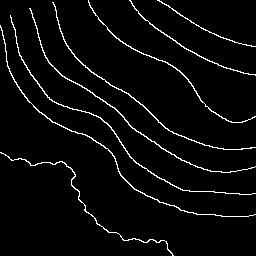
\includegraphics[width=1\textwidth, valign=c]{images/5_label.png}
        \caption{}
    \end{subfigure}
    \begin{subfigure}[t]{0.24\textwidth}
        \centering
        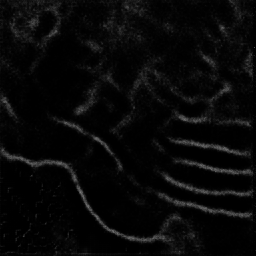
\includegraphics[width=1\textwidth, valign=c]{images/segnet_5_predict.png}
        \caption{}
        \label{fig:segexample}
    \end{subfigure}
    \begin{subfigure}[t]{0.24\textwidth}
        \centering
        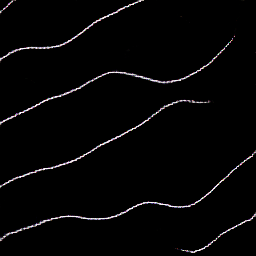
\includegraphics[width=1\textwidth, valign=c]{images/pix2pix_predict.png}
        \caption{}
        \label{fig:pixexample}
    \end{subfigure}
    \caption{Example predictions produced by the SegNet architecture and the pix2pix model. \textbf{(a)} The original coral skeleton patch. \textbf{(b)} The corresponding ground truth label. \textbf{(c)} A prediction output by the SegNet architecture. Although some banding is correctly identified in the bottom right of the prediction, the qualitative performance is poor overall. \textbf{(d)} A label generated by the pix2pix model. Although the generated boundaries are continuous, smooth, and sharp, they do not follow the same direction as the ground truth boundaries and are too far apart.}
    \label{fig:segpixexample}
\end{figure}

\section{Evaluation}

\subsection{Boundary Extraction}

The majority of the project focused on the use of deep neural networks to extract the annual density band boundaries present in coral skeletons. This section aims to evaluate the decisions made throughout the project regarding this extraction process.

\subsubsection{Labelling Method}
\label{sec:evallabel}

It has been mentioned that the utilised labelling method gives rise to a severe class imbalance which introduces challenges when assessing performance. Although the goal of this project was to extract the boundaries between density bands, a labelling method in which the bands themselves were labelled might have been more a sensible choice. In this method, the possible classes would instead be ``part of a high density band'' and ``part of a low density band''. Since the high and low density bands are roughly equal in width, this labelling method would enable the number of pixels classified as a high band to be roughly equal to the number of pixels classified as a low band. As a result, the class imbalance within the labels would be significantly reduced and a standard per-pixel accuracy could be used.

Since the U-Net architecture is also capable of classifying more than two classes, the use of a third class to represent the area outside of a coral skeleton may have been useful. The current labelling method treats the growth surface of a skeleton as a density band boundary, even though this is technically not the case. The performance of the network in classifying banding boundaries may currently be hindered by the need to also classify the growth surface as a banding boundary, even though the nature of a growth surface is significantly different to the nature of an actual boundary.

\subsubsection{Lack of Labelled Data}

The experiments carried out in Section \ref{sec:evalaugmentation} involving data augmentation highlighted the effect that the lack of labelled data has on performance. An increase in the amount of labelled data would reduce the need for as many regularization techniques and would most likely increase the performance achieved. The lack of labelled data available is mostly due to the challenges involved in the manual labelling process. As mentioned in Chapter \ref{chap:implementation}, upon visual inspection of over 50 Porites scans, only four scans contained slices that could be labelled confidently. Although more slices were labelled to be used by the three dimensional architecture, these slices were from the same scans and the labelling across adjacent slices was not consistent.

When this boundary extraction task is revisted, a larger amount of consistently labelled data will be key in improving the performance achieved.

\subsubsection{Three Dimensional Architectures}

Seeing as the two dimensional augmentation proved so important, it stands to reason that the performance achieved by an architecture making use of three dimensional data would also benefit significantly from appropriate augmentation. Although some forms of augmentation such as rotations, flips, and brightness shifts were implemented, the implementation of further transformations such as shifts, shearing, and zooming could have improved the performance achieved by the architectures that made use of a third dimension.

As mentioned in Section \ref{sec:eval3darch}, the inconsistent labelling of the adjacent slices that compose the three dimensional data was a problem. In hindsight, perhaps each slice should have been labelled whilst constantly referencing the label of an adjacent slice, in order to ensure that the labelling is consistent in the third dimension. Although this labelling process would take appreciably more time per slice, it could potentially improve the performance achieved by both the two and three dimensional architectures significantly.

\subsection{Accuracy Metric}
\label{sec:evalaccuracy}

The custom accuracy metric played a significant role in assessing the performance achieved by the various networks experimented with. Although the metric does solve many of the problems faced by a classic per-pixel accuracy metric, it is not without its issues.

The most obvious shortcoming highlighted in Section \ref{sec:evalablation}, is the fact that breaks in continuity are not punished enough. Breaks in continuity are indirectly punished to some extent, since a break results in the corresponding area of a ground truth boundary having no pixels close to it. However, the continuity of the boundaries is essential for the estimation of the calcification rate and should thus contribute to the accuracy achieved far more than it does currently.

Although the accuracy often reflects the qualitative performance well, there are examples in which visual inspection is still required to assess the performance of the network on this task. For example, although the predictions shown previously in Figure \ref{fig:ablation} vary noticeably in terms of quality, the accuracy achieved by all of the predictions were within ${\sim}3\%$ of each other.

It is important to note that despite its shortcomings, there is a still a clear correlation between the qualitative performance observed and the accuracy metric achieved. The custom accuracy metric is far more useful than a standard per-pixel accuracy, and it has enabled useful quantitative comparisons to be made throughout the project.

% \subsection{Calcification Rate Estimation}

% Although the automatic calcification rate estimations were similar to the manual estimates reported in the literature, the method used in this project is not fully automated. Ideally, the two points specifying which area to estimate within would not have to be specified. If the labelling method outlined in Section \ref{sec:evallabel} was utilised (in which the outside of a coral is labelled as a different class), a fully automatic method could potentially be implemented. The method could, for example, start from the outside of the skeleton and using work its way in, keeping track of the distances between boundaries as it goes.

% Ideally two points would not have to be supplied and the solution would find the outside and work its way in. would perhaps be possible with 3 classes.

% Rather than just using a thin rectangular area, a larger area could have been used allowing more point samples?

% {\bf A topic-specific chapter, of roughly $15$ pages} 
% \vspace{1cm} 

% \noindent
% This chapter is intended to evaluate what you did.  The content is highly 
% topic-specific, but for many projects will have flavours of the following:

% \begin{enumerate}
% \item functional  testing, including analysis and explanation of failure 
%       cases,
% \item behavioural testing, often including analysis of any results that 
%       draw some form of conclusion wrt. the aims and objectives,
%       and
% \item evaluation of options and decisions within the project, and/or a
%       comparison with alternatives.
% \end{enumerate}

% \noindent
% This chapter often acts to differentiate project quality: even if the work
% completed is of a high technical quality, critical yet objective evaluation 
% and comparison of the outcomes is crucial.  In essence, the reader wants to
% learn something, so the worst examples amount to simple statements of fact 
% (e.g., ``graph X shows the result is Y''); the best examples are analytical 
% and exploratory (e.g., ``graph X shows the result is Y, which means Z; this 
% contradicts [1], which may be because I use a different assumption'').  As 
% such, both positive {\em and} negative outcomes are valid {\em if} presented 
% in a suitable manner.